% This is file NWSguide.tex
% release v1.00, 12th June 2012
%   (based on JFPguide.tex v1.11 for LaTeX 2.09)
% Copyright (C) 2012 Cambridge University Press

\NeedsTeXFormat{LaTeX2e}

\documentclass{nws}

%%% Macros for the guide only %%%
\providecommand\AMSLaTeX{AMS\,\LaTeX}
\newcommand\eg{\emph{e.g.}\ }
\newcommand\etc{\emph{etc.}}
\newcommand\bcmdtab{\noindent\bgroup\tabcolsep=0pt%
  \begin{tabular}{@{}p{10pc}@{}p{20pc}@{}}}
\newcommand\ecmdtab{\end{tabular}\egroup}
\newcommand\rch[1]{$\longrightarrow\rlap{$#1$}$\hspace{1em}}
\newcommand\lra{\ensuremath{\quad\longrightarrow\quad}}

\title[Network Science]
      {\LaTeXe\ guide for Network Science}

 \author[D.A. Tranah]
        {David Tranah\\
         Cambridge University Press, Cambridge CB2 2RU, UK\\
         \email{dtranah@cambridge.org}}

\jdate{June 2012}
\pubyear{2012}
\pagerange{\pageref{firstpage}--\pageref{lastpage}}
\doi{S0956796801004857}

\newtheorem{lemma}{Lemma}[section]

\begin{document}

\label{firstpage}

\maketitle

\begin{abstract}
This guide is for authors who are preparing papers for \emph{Network Science}
 using the \LaTeXe\ document-preparation system
and the Network Science class file (\texttt{nws.cls}).
\end{abstract}

\tableofcontents

\section{Introduction}

Newtork Science accepts submissions either in Microsoft Word or in \LaTeX\ format.
This guide describes the use and features of the class for the journal. It is
based on the \verb"article"
class as discussed in the \LaTeX\ manual (2nd edition) \cite{LaTeX}.
Commands which differ from the standard \LaTeXe\ interface, or which are
provided in addition to the standard interface, are explained in this
guide (which is \emph{not} a substitute for the \LaTeXe\ manual itself).
We assume you are already familiar with \LaTeX.

Note that this guide uses the public \verb"mathptmx" fonts. If you use this guide
as a template please note that
the final printed version of papers may use a different typeface
so line and page breaks will change. Therefore do not put hard page or line breaks into the document

Authors planning to submit their papers in \LaTeXe\ are advised to use
\verb"nws.cls" as early as possible in the creation of their files.

\subsection{Introduction to \LaTeX}

\LaTeX\ is constructed as a series of macros on top of the \TeX\ typesetting
program. \LaTeX\ adds to \TeX\ a collection of facilities which simplify
typesetting for authors by allowing them to concentrate on the logical
structure of the document rather than its visual layout. Careful use of the
\LaTeX\ mark-up philosophy results in uniform layout rather than the
\emph{ad hoc} results of some word-processing systems. Authors are advised to
let the defaults control font selection etc., rather than tinker themselves.

The \LaTeX\ system provides a consistent and comprehensive document preparation
interface. Among other things, \LaTeX\ can automatically number list
entries, equations, figures, tables and footnotes, as well as sections and
subsections. Using this numbering system, bibliographic citations, page
references and cross references to any other numbered entity (e.g. sections,
equations, figures) are straightforward.

\subsection{The NWS document class}

The use of document classes allows a simple change of style (or style option)
to transform the appearance of your document. The NWS class preserves the
standard \LaTeX\ interface such that any document which can be produced
using the standard \LaTeX\ \verb"article" class can also be produced with
the NWS class.

\subsection{General style issues}

Use of \LaTeX\ defaults will result in a pleasing uniformity of layout
and font selection. Authors should resist the temptation to make
\emph{ad hoc} changes to these. Also avoid use of direct formatting unless
really necessary. Papers will be edited as usual, and this process may be
obstructed by the use of inserted line breaks, etc.

For general style issues, authors are referred to the `Preparation of
manuscripts' in the back cover of the journal. Authors who are interested in
the details of style are referred to \cite{Butcher} and \cite{Chicago}. The
language used in the journal is US English, and spelling should conform
to this.

Use should be made of symbolic references (\verb"\ref") in order to
protect against late changes of order, etc.

\subsection{Submission of \LaTeX\ articles}

Authors who intend to submit a \LaTeX\ article should obtain a copy of the
NWS class file. This is available by anonymous FTP from
%
\begin{verbatim}
  ftp.cup.cam.ac.uk
\end{verbatim}
%
You will find the class file and instructions contained in a
single file \verb"nwscls.ltx" in the directory
%
\begin{verbatim}
  pub/texarchive/journals/latex/nws-cls
\end{verbatim}
%
The \verb"readme.txt" (which is the same directory) tells you how to
unpack the file \verb"nwscls.ltx".
There may also be an `\verb"unpacked"' directory containing all of the files
separately, in case of difficulty. If you cannot obtain the NWS files,
use the standard \verb"article" class, with the default `\verb"10pt"' option.

When submitting the final article, ensure that  the following are included and
are clearly labelled.
\begin{enumerate}
  \item A hardcopy printout of the article.
  \item The input file (exactly matching the hardcopy).
  \item A copy of any user-defined macros.
  \item If you have used \textsc{Bib}\TeX, the \verb".bib", \verb".bbl"
        and \verb".bst" files that were used.
  \item Any other files necessary to prepare the article for typesetting.
\end{enumerate}
The files for the \emph{final} article should be text-only with no
system-dependent control codes.

\section{Using the NWS class file}
\label{usingjnwsclass}

First, copy the file \verb"nws.cls" (and \verb"nws.bst" if you use Bib\TeX)
into an appropriate subdirectory on your system. The NWS class is implemented
as a complete document class, and \emph{not} as an class option.
In order to use the NWS class, replace \verb"article" by \verb"nws" in the
\verb"\documentclass" command at the beginning of your document: that is,
%
\begin{verbatim}
  \documentclass{article}
\end{verbatim}
%
is replaced by
%
\begin{verbatim}
  \documentclass{nws}
\end{verbatim}
%
Author-defined macros should be inserted before \verb"\begin{document}",
or in a separate file and should be included with the submission.
Authors must not change any of the macro definitions or parameters
in \verb"nws.cls".


\subsection{Document class options}\label{sec:ClassOp}

In general, the following standard document class options should \emph{not} be
used with the NWS class file:
%
\begin{itemize}
  \item \texttt{10pt}, \texttt{11pt} and \texttt{12pt} -- unavailable;
  \item \texttt{twoside} is the default (\texttt{oneside} is disabled);
  \item \texttt{onecolumn} is the default (\texttt{twocolumn} is disabled);
  \item \texttt{titlepage} is not required and is disabled;
  \item \texttt{fleqn} and \texttt{leqno} should not be used, and are disabled.
\end{itemize}
%
\ifprodtf
The following new class options are provided:
\begin{itemize}
  \item \texttt{prodtf} -- tells the class file that we want to use the
    production typeface. This automatically sets the odd, even and top
    margins.
\end{itemize}
\fi

\section{Additional facilities}

In addition to all the standard \LaTeX\ design elements, the NWS class
includes the following features.
%
\begin{itemize}
  \item Additional commands for typesetting the title page. Extended
        commands for specifying a short version of the title and author(s)
        for the running headlines.
  \item New options to the \verb"\maketitle" command to create Functional and
        Theoretical Pearl(s).
  \item A \verb"proof" environment.
%  \item A \verb"capsule" environment for typesetting Capsule Reviews.
  \item Control of enumerated lists.
\end{itemize}
%
Once you have used these additional facilities in your document,
it can be processed only with \verb"nws.cls".

\subsection{Titles, authors' names and running headlines}

At the beginning of your article, the title should be generated in the
usual way using the \verb"\maketitle" command. Immediately following the
title you may include an abstract and/or capsule review. For example, the titles
for this guide were produced by the following source.
%
\begin{verbatim}
  \title[Network Science]
        {\LaTeXe\ guide for Network Science}
  \author[D.A. Tranah]
         {David Tranah\\
          Cambridge University Press, Cambridge CB2 2RU, UK\\
          \email{dtranah@cup.cam.ac.uk}}
\end{verbatim}

\verb"\begin{document}"\\
\indent\verb"\maketitle"

\begin{verbatim}
  \begin{abstract}
  This guide is for authors who are preparing papers...
  \end{abstract}
\end{verbatim}

In the NWS class, the title of the article and the author's name (or
authors' names) are used both at the beginning of the article for the main
title and throughout the article as running headlines at the top of every
page. The title is used on odd-numbered pages (rectos) and the author's name
appears on even-numbered pages (versos). The \verb"\pagestyle" and
\verb"\thispagestyle" commands should \emph{not} be used.  Similarly, the
commands \verb"\markright" and \verb"\markboth" should not be necessary.

Although the article title can run to several lines of text, the running
headline must be a single line. Moreover, the title can incorporate new-line
commands (e.g. \verb"\\"), but these are not acceptable in a running headline.
To enable you to specify an alternative short title, and an alternative short
author's name, the standard \verb"\title" and \verb"\author" commands have
been extended to take an optional argument to be used as the running headline.
%
\begin{verbatim}
  \title[Short title]
        {Full title which can be as long as necessary}
  \author[Author name]
         {AUTHOR NAME \\ Affiliation}
\end{verbatim}
%
Notice that the author name in the argument for the running head should
be in mixed case, and the author name for the title should be in upper
case only. The author affiliation is set in the normal way, after a
\verb"\\" in the argument to the \verb"\author" command.

Any `work supported by' or `authors current address' information should
be inserted via \verb"\thanks" commands, which should be positioned
after the appropriate `AUTHOR NAME' in the \verb"\author" command.

If there are four (or more) authors for the article, the author running head
should contain the first author name followed by `et~al.' only. e.g.
%
\begin{verbatim}
  \author[Author1 et al.]
         {AUTHOR1...}
\end{verbatim}

The previous examples show an article with one author, the normal
\LaTeX\ conventions have been extended to allow the author names and
their affiliations to be typeset in the correct NWS style. The following
examples should cover most possibilities:

\textit{Case 1.} Two authors with the same affiliation:
%
\begin{verbatim}
  \author[Author1 and Author2]
         {AUTHOR1 and AUTHOR2\\
          Affiliation for both authors}
\end{verbatim}
%
If the author names are too long to fit onto one line, it should be
broken into two or more lines using the \verb"\authorbreak" command.
Don't use \verb"\\" to linebreak the author names -- as this will not do what
you expect.

\textit{Case 2.} Two authors with different affiliations:
%
\begin{verbatim}
  \author[Author1 and Author2]
         {AUTHOR1\\
          Affiliation for Author1
          \and AUTHOR2\\
          Affiliation for Author2}
\end{verbatim}

\textit{Case 3.} Three (or more) authors, two with the same affiliation:
%
\begin{verbatim}
  \author[Author1, Author2 and Author3]
         {AUTHOR1, AUTHOR2\\
            Affiliation for Author1 and Author2
          \and AUTHOR3\\
            Affiliation for Author3}
\end{verbatim}

\subsection{Proofs}

A new environment exists for creating Proofs, e.g.
%
\begin{proof}
  Use $K_\lambda$ and $S_\lambda$ to translate combinators
  into $\lambda$-terms. For the converse, translate
  $\lambda x$ \ldots by [$x$] \ldots and use induction
  and the lemma.
\end{proof}
%
This was produced by the following code:
%
\begin{verbatim}
  \begin{proof}
    Use $K_\lambda$ and $S_\lambda$ to...
  \end{proof}
\end{verbatim}
%
The end of proof marker \proofbox\ is produced automatically. If you wish
to omit this, use the \verb"proof*" environment instead.

If a proof ends with a display equation, then it is customary for the proofbox
to be positioned at the end of equation finishing the proof. \eg
%
\begin{proof*}
  Use $K_\lambda$ and $S_\lambda$ to translate combinators
  into $\lambda$-terms. For the converse, translate
  $\lambda x$ \ldots by [$x$] \ldots and use induction
  and the lemma.
  \[ a_1 \equiv (2\Omega M^2/x) \mathproofbox \]
\end{proof*}
%
Was produced with:
%
\begin{verbatim}
  \begin{proof*}
    Use $K_\lambda$ and $S_\lambda$ to...
    \[ a_1 \equiv (2\Omega M^2/x) \mathproofbox \]
  \end{proof*}
\end{verbatim}
%
Notice the use of \verb"proof*" to turn off the automatic proofbox.

The proof environment will also take an optional argument which allows you
to produce `special' proofs. e.g.
%
\begin{proof}[Proof of Theorem 27]
  We define a linear isometry $A:H\rightarrow H$ by the nonlinear
  Schr\"{o}dinger equation. It would not be hard to modify the
  proof to obtain an analogous result for ellipsoids rather than
  spheres.
\end{proof}
%
Which was produced like this:
%
\begin{verbatim}
  \begin{proof}[Proof of Theorem 27]
    We define a linear isometry...
  \end{proof}
\end{verbatim}
%
Notice that once the optional argument is used, you have to type all of
the text which is to appear as the heading.

\subsection{Figures}

The NWS class will cope with most positioning of your figures. 
As captions fall below figures, the figure must be included first, then the caption, 
then the label. This is illustrated in Figure~\ref{cantor}. The \verb"cantor1.eps" file has been 
called in by using \verb"\usepackage{graphicx}" in the preamble. Note that if you are producing 
a list of illustrations (using \verb"\listoffigures"), you need to repeat the caption in square 
braces, but without the full point.
  \begin{figure}
    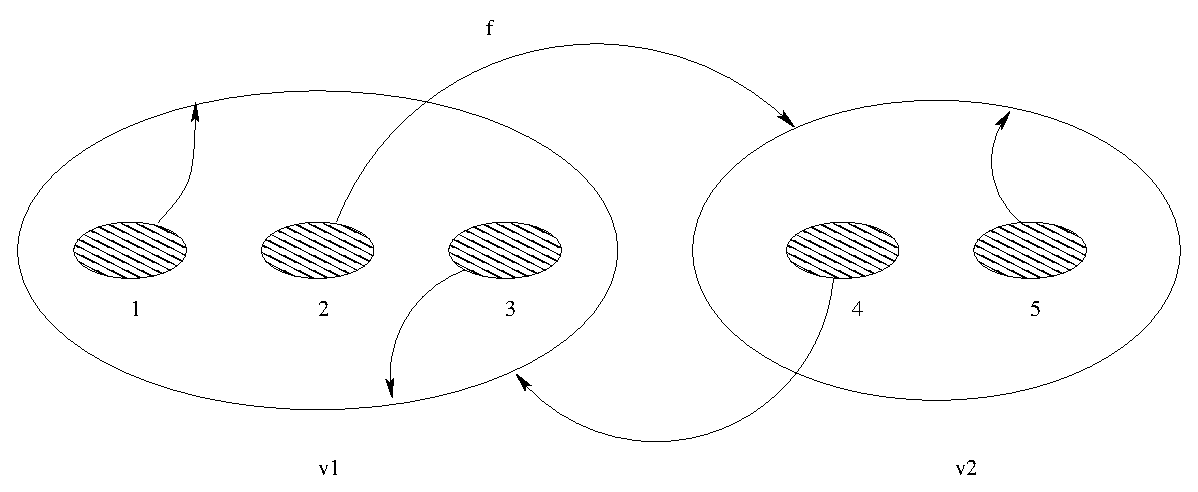
\includegraphics[scale=0.55]{cantor1.eps}
    %  note that the square brace option below is only required
    %  if you intend to produce a list of illustrations
    \caption[Shortened figure caption for the list of illustrations]
      {A Cantor repeller. Long figure captions will be indented left
      and right; short ones will be centred by default.}
    \label{cantor}
\rule[-20pt]{\textwidth}{0.6pt}
\begin{verbatim}
  \begin{figure}
    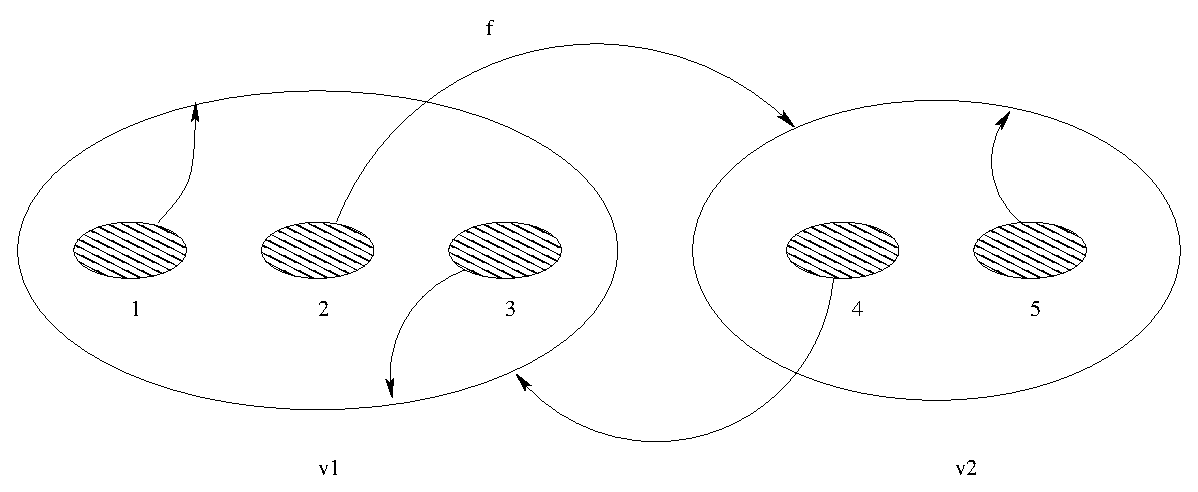
\includegraphics[scale=0.55]{cantor1.eps}
    %  note that the square brace option below is only required
    %  if you intend to produce a list of illustrations
    \caption[Shortened figure caption for the list of illustrations]
      {A Cantor repeller. Long figure captions will be indented left
      and right; short ones will be centred by default.}
    \label{cantor}
  \end{figure}
\end{verbatim}
\rule[20pt]{\textwidth}{0.5pt}
  \end{figure}

\subsection{Programs}\label{sec-programs}

NWS encourages authors to use one of two styles for typesetting programs,
\emph{mathematical} and \emph{verbatim}.

A program typeset in the mathematical style is shown in
Figure~\ref{mathfigure}, and the commands used to typeset this program
are shown in Figure~\ref{mathtypeset}.  This uses the ordinary
mathematics mode of \LaTeX: displayed programs are surrounded by
\verb|\[| and \verb|\]|, and the \verb|array| command is used for
alignment.  However, there are two important differences.  First, the
\verb|\programmath| command appears before the program text; this
causes math mode to use ordinary spacing for italic identifiers,
rather than math spacing.  The \verb|\unprogrammath| command returns
to normal math spacing.  Second, in math mode spaces are ignored, so a
tilde \verb|~| is used instead.  (In \LaTeX, a tilde generates a
``hard space'' that is never replaced by a line break.)  To include
program text in mathematics style inline, surround it with dollar
\verb|$| signs.  For example, the input
\begin{verbatim}
  See how \programmath $differ~x$
  differs from \unprogrammath $differ x$.
\end{verbatim}
produces the output
\begin{center}
  See how \programmath $differ~x$
  differs from \unprogrammath $differ x$.
\end{center}

A program typeset in the verbatim style is shown in
Figure~\ref{verbfigure}, and the commands used to typeset this program
are shown in Figure~\ref{verbtypeset}.  This uses the ordinary
verbatim mode of \LaTeX: displayed programs are surrounded by
\verb|\begin{verbatim}| and \verb|\end{verbatim}|, and alignment is
indicated with spaces in the source file (don't use tabs, which may
not be processed properly).  To include program
text in verbatim style inline, use the \verb|\verb| command.
For example, the input
\begin{center}
\begin{verbatim}
  On a terminal, this looks like \verb"differ x".
\end{verbatim}
\end{center}
produces the output
\begin{center}
  On a terminal, this looks like \verb"differ x".
\end{center}

It is recommended that programs in figures be offset from the text
using the \verb|\figrule| command, as shown in Figures~\ref{mathfigure}%
--\ref{verbtypeset}.

\begin{figure}
\figrule
\programmath
\[
\begin{array}{lcl}
exp                   & :: & Exp \rightarrow Arr \rightarrow Val \\
exp~(Var~i)~a         & =  & index~i~a \\
exp~(Const~v)~a       & =  & v \\
exp~(Plus~e_1~e_2)~a  & =  & exp~e_1~a+exp~e_2~a \\
\\
com                   & :: & Com \rightarrow Arr \rightarrow Arr \\
com~(Asgn~i~e)~a      & =  & update~i~(exp~e~a)~a \\
com~(Seq~c_1~c_2)~a   & =  & com~c_2~(com~c_1~a) \\
com~(If~e~c_1~c_2)~a  & =  & \textrm{if } exp~e~a \dequals 0 \textrm{ then }
                                      com~c_1~a \textrm{ else } com~c_2~a \\
\\
prog                  & :: & Prog \rightarrow Val\\
prog~(Prog~c~e)       & =  & exp~e~(com~c~(newarray~0))
\end{array}
\]
\unprogrammath
\caption{Example program in mathematical style.}\label{mathfigure}
\figrule
\begin{center}
\begin{verbatim}
\begin{figure}
\figrule
\programmath
\[
\begin{array}{lcl}
exp                   & :: & Exp \rightarrow Arr \rightarrow Val \\
exp~(Var~i)~a         & =  & index~i~a \\
exp~(Const~v)~a       & =  & v \\
exp~(Plus~e_1~e_2)~a  & =  & exp~e_1~a+exp~e_2~a \\
\\
com                   & :: & Com \rightarrow Arr \rightarrow Arr \\
com~(Asgn~i~e)~a      & =  & update~i~(exp~e~a)~a \\
com~(Seq~c_1~c_2)~a   & =  & com~c_2~(com~c_1~a) \\
com~(If~e~c_1~c_2)~a  & =  & \textrm{if } exp~e~a \dequals 0 \textrm{ then }
                                      com~c_1~a \textrm{ else } com~c_2~a \\
\\
prog                  & :: & Prog \rightarrow Val\\
prog~(Prog~c~e)       & =  & exp~e~(com~c~(newarray~0))
\end{array}
\]
\unprogrammath
\caption{Example program in mathematical style.}\label{mathfigure}
\figrule
\end{verbatim}
\end{center}
\caption{Typesetting the example program in mathematical style.}\label{mathtypeset}
\figrule
\end{figure}

\begin{figure}
\figrule
\begin{verbatim}
  exp                 :: Exp -> Arr -> Val
  exp (Var i) a       =  index i a
  exp (Const v) a     =  v
  exp (Plus e1 e2) a  =  exp e1 a + exp e2 a

  com                 :: Com -> Arr -> Arr
  com (Asgn i e) a    =  update i (exp e a) a
  com (Seq c1 c2) a   =  com c2 (com c1 a)
  com (If e c1 c2) a  =  if  exp e a == 0  then  com c1 a  else  com c2 a

  prog                :: Prog -> Val
  prog (Prog c e)     =  exp e (com c (newarray 0))
\end{verbatim}
\caption{Example program in verbatim style.}\label{verbfigure}
\figrule
\begin{tabular}{l}
\verb|\begin{figure}| \\
\verb|\figrule| \\
\verb|\begin{center}| \\
\verb|\begin{verbatim}| \\
\verb|exp                 :: Exp -> Arr -> Val| \\
\verb|exp (Var i) a       =  index i a| \\
\verb|exp (Const v) a     =  v| \\
\verb|exp (Plus e1 e2) a  =  exp e1 a + exp e2 a| \\
\\
\verb|com                 :: Com -> Arr -> Arr| \\
\verb|com (Asgn i e) a    =  update i (exp e a) a| \\
\verb|com (Seq c1 c2) a   =  com c2 (com c1 a)| \\
\verb|com (If e c1 c2) a  =  if  exp e a == 0  then  com c1 a  else  com c2 a| \\
\\
\verb|prog                :: Prog -> Val| \\
\verb|prog (Prog c e)     =  exp e (com c (newarray 0))| \\
\verb|\end{verbatim}| \\
\verb|\end{center}| \\
\verb|\caption{Example program in verbatim style.}\label{verbfigure}| \\
\verb|\figrule| \\
\verb|\end{figure}|
\end{tabular}
\caption{Typesetting the example program in verbatim style.}\label{verbtypeset}
\figrule
\end{figure}

Some new macros have been provided for a few convenient symbols in
math mode.  These are illustrated in Table~\ref{newcommands}.
\ifprodtf\newpage\fi

\begin{table}
\caption{New symbol macros}\label{newcommands}
\programmath
\begin{tabular}{lll}
\hline\hline
Symbol                & Usage                  & Keyed as\\
\hline
\verb"\dplus"         & $abc \dplus xyz$         & \verb"$abc \dplus xyz$"\\
\verb"\dequals"       & $abc \dequals xyz$       & \verb"$abc \dequals xyz$"\\
\verb"\dcolon"        & $abc \dcolon xyz$        & \verb"$abc \dcolon xyz$"\\
\verb"\dcolonequals"  & $abc \dcolonequals xyz$  & \verb"$abc \dcolonequals xyz$"\\
\hline\hline
\end{tabular}
\unprogrammath
\end{table}

\subsection{Abstract and Capsule reviews}

The NWS class provides for an abstract and/or a capsule review; the
abstract is produced by the following commands:
%
\begin{verbatim}
  \begin{abstract}
       :
  \end{abstract}
\end{verbatim}
%
whereas the capsule review is produced by:
%
\begin{verbatim}
  \begin{capsule}
       :
  \end{capsule}
\end{verbatim}
%
Either or both of these may be used, in either order, but it is assumed
that, if both are used, there will be no other material between them.
In NWS the abstract should precede any capsule review.

\subsection{Lists}

The NWS class provides the three standard list environments.
\begin{itemize}
  \item Numbered lists, created using the \verb"enumerate" environment;
  \item Bulleted lists, created using the \verb"itemize" environment;
  \item Labelled lists, created using the \verb"description" environment.
\end{itemize}
The \verb"enumerate" environment numbers each list item with an arabic numeral;
alternative styles can be achieved by inserting a redefinition of the
number labelling command after the \verb"\begin{enumerate}". For example, a
list numbered with roman numerals inside parentheses can be produced by the
following commands:
%
\begin{verbatim}
  \begin{enumerate}[(iii).]
    \renewcommand{\theenumi}{(\roman{enumi})}
    \item first item
          :
  \end{enumerate}
\end{verbatim}
%
This produces the following list:
%
\begin{enumerate}[(iii).]
  \renewcommand{\theenumi}{(\roman{enumi})}
  \item first item
  \item second item
  \item \etc
\end{enumerate}
%
Notice that an optional argument ``\verb"(iii)."'' has been given to the
\verb"enumerate" environment, specifying the \emph{widest label} used in the
list. This is because roman numerals are wider than the arabic numerals
normally used by \verb"enumerate", and so the labels would otherwise have been
pushed out into the margin.

\section{User-defined macros}

If you define your own macros, you must ensure that their names do not
conflict with any existing macros in \LaTeX\ (or \AMSLaTeX\ %
if you are using this). You should also place them in the preamble of
your input file, between the \verb"\documentclass" (but after any
\verb"\usepackage" commands) and before the \verb"\begin{document}" command.

Apart from scanning the indexes of the relevant manuals, you can check
whether a macro name is already used by using \verb"\newcommand", which
will check for the existence of the macro you are trying to define.
If the macro exists \LaTeX\ will respond with:
%
\begin{verbatim}
  ! LaTeX Error: Command ... already defined.
\end{verbatim}
%
In this case you should choose another name, and try again.

Such macros must be in a place where they can easily be found and
modified by the journal's editors or typesetter. They must be gathered
together in the preamble of your input file, or in a separate
\verb"macros.tex" file with the command \verb"\input{macros}" in the
preamble. Macro definitions must not be scattered about your document
where they are likely to be completely overlooked by the typesetter.

The same applies to font definitions that are based on Computer Modern
fonts. These must be changed by the typesetter to use the journal's
correct typeface. In this case, you should draw
attention to these font definitions on the hard copy that you submit for
publication and by placing a comment in your input file just before the
relevant definitions, for example \verb"% replace font!"

\section{Some guidelines for using standard facilities}

The following notes may help you achieve the best effects with the NWS class file.

\subsection{Sections}

\LaTeX\ provides five levels of section headings and they are all
defined in the NWS class file:
\begin{itemize}
  \item[] Heading A -- \verb"\section{...}"
  \item[] Heading B -- \verb"\subsection{...}"
  \item[] Heading C -- \verb"\subsubsection{...}"
  \item[] Heading D -- \verb"\paragraph{...}"
  \item[] Heading E -- \verb"\subparagraph{...}"
\end{itemize}
Section numbers are given for sections, subsection and subsubsection headings.

\subsection{Figures and tables}

The \texttt{figure} and \texttt{table} environments are implemented as described in
the \LaTeX\ Manual to
provide consecutively numbered floating inserts for illustrations and tables
respectively.
The standard inserts and their captions are formatted centred.
Line breaks in captions can be inserted as required using \verb"\\".

\subsubsection{Illustrations (or figures)}

The NWS class will cope with most positioning of your illustrations
and you should not normally use the optional positional qualifiers on
the \verb"figure" environment which would override these decisions.
Figure captions should be below the figure itself, therefore the
\verb"\caption" command should appear after the figure or space left
for an illustration.

Some figures in NWS will illustrate programs, as shown in
Section~\ref{sec-programs} of this guide. Figure~\ref{sample-figure}
shows an example of space left above a caption for artwork to be pasted in.
This was produced with the following commands:
%
\begin{verbatim}
  \begin{figure}
    \vspace{5cm} % the vertical depth of the artwork
    \caption{An example figure with space for artwork.}
    \label{sample-figure}
  \end{figure}
\end{verbatim}
%
\begin{figure}
  \vspace{5cm} % the vertical depth of the artwork
  \caption{An example figure with space for artwork.}
  \label{sample-figure}
\end{figure}
%
The vertical depth should correspond roughly to the artwork you will submit;
it will be adjusted to fit the final artwork exactly.

If your illustration extends over two~pages, you can use the
\verb"\continuedfigure" facility. To use this, you key the figure
caption for the second figure as follows:
%
\begin{verbatim}
  \begin{figure}
    \continuedfigure
    \vspace{80pt}
    \caption{First figure, continued.}
    \label{continued}
  \end{figure}
\end{verbatim}
%
This ensures that the figure counter does not get incremented, and at the
same time adds the word (cont.) to the caption. You may still use labels
and references for this figure.

\subsubsection{Tables}

The NWS class file will cope with most positioning of your tables
and you should not normally use the optional positional qualifiers on the
\verb"table" environment which would override these decisions.
Normal journal style sets the table caption first, followed by a double
rule, the table body and a double rule at the bottom. Single rules and
spanner rules (\verb"\cline") can be used to separate headings from the
columns. For example, Table~\ref{sample-table} is produced using the
following commands:\par
%
{\small
\begin{verbatim}
\begin{table}
  \caption{Results of Overloading for 3 Experimental Setups}
  \label{sample-table}
  \begin{minipage}{\textwidth}
    \begin{tabular}{lcrrrrr}
      \hline\hline
      Program& Expt.&
      CPU\footnote{Seconds of elapsed time on an unloaded Sun 3/50.}&
      RelCPU\footnote{CPU Time relative to experiment (a).}& GC&
      Mem\footnote{Bytes of heap used over the duration of the program.}&
      RelMem\footnote{Memory usage relative to experient (a).}\\
      \hline
      8 Queens& (a)&   2.88&  1.00&    6&   1.7M&  1.00\\
      &         (b)&  32.51& 11.29&  193&  48.9M& 28.76\\
      &         (c)&   7.90&  2.74&   42&  11.3M&  6.65\\
      \noalign{\vspace {.5cm}}
      Primes&   (a)&   4.89&  1.00&   19&   5.3M&  1.00\\
      &         (b)&  47.54&  9.72&  204&  54.5M& 10.28\\
      &         (c)&  10.08&  2.06&   47&  13.0M&  2.45\\
      \noalign{\vspace {.5cm}}
      Nfib&     (a)&  21.65&  1.00&  161&  40.4M&  1.00\\
      &         (b)& 221.65& 10.24& 1382& 349.0M&  8.64\\
      &         (c)&  21.30&  0.98&  161&  42.0M&  1.03\\
      \noalign{\vspace {.5cm}}
      KWIC&     (a)&   7.07&  1.00&   15&   6.3M&  1.00\\
      &         (b)&  34.55&  4.89&  109&  47.8M&  7.59\\
      &         (c)&  31.62&  4.47&   53&  45.0M&  7.14\\
      \hline\hline
    \end{tabular}
    \vspace{-2\baselineskip}
  \end{minipage}
\end{table}
\end{verbatim}}
%
\begin{table}
  \caption{Results of Overloading for 3 Experimental Setups}
  \label{sample-table}
  \begin{minipage}{\textwidth}
    \begin{tabular}{lcrrrrr}
      \hline\hline
      Program& Expt.&
      CPU\footnote{Seconds of elapsed time on an unloaded Sun 3/50.}&
      RelCPU\footnote{CPU Time relative to experiment (a).}& GC&
      Mem\footnote{Bytes of heap used over the duration of the program.}&
      RelMem\footnote{Memory usage relative to experient (a).}\\
      \hline
      8 Queens& (a)&   2.88&  1.00&    6&   1.7M&  1.00\\
      &         (b)&  32.51& 11.29&  193&  48.9M& 28.76\\
      &         (c)&   7.90&  2.74&   42&  11.3M&  6.65\\
      \noalign{\vspace {.5cm}}
      Primes&   (a)&   4.89&  1.00&   19&   5.3M&  1.00\\
      &         (b)&  47.54&  9.72&  204&  54.5M& 10.28\\
      &         (c)&  10.08&  2.06&   47&  13.0M&  2.45\\
      \noalign{\vspace {.5cm}}
      Nfib&     (a)&  21.65&  1.00&  161&  40.4M&  1.00\\
      &         (b)& 221.65& 10.24& 1382& 349.0M&  8.64\\
      &         (c)&  21.30&  0.98&  161&  42.0M&  1.03\\
      \noalign{\vspace {.5cm}}
      KWIC&     (a)&   7.07&  1.00&   15&   6.3M&  1.00\\
      &         (b)&  34.55&  4.89&  109&  47.8M&  7.59\\
      &         (c)&  31.62&  4.47&   53&  45.0M&  7.14\\
      \hline\hline
    \end{tabular}
    \vspace{-2\baselineskip}
  \end{minipage}
\end{table}

Notice the use of the `\verb"\vspace{-2\baselineskip}"' command to remove the
unwanted vertical space from above the table footnotes in this example.

Captions for `continued' tables can be generated (in the same way as for figures)
using the \verb"\continuedtable" command. These should be positioned just before
the \verb"\caption" command in the appropriate table environment.

The \verb"tabular" environment should be used to produce ruled tables;
it has been modified for the NWS class in the following ways:
\begin{enumerate}
  \item Additional vertical space is inserted above and below a horizontal rule
        (produced by \verb"\hline");
  \item Tables are centred, and span the full width of the page; that is,
  they are similar to the tables that would be produced by
  \verb"\begin{minipage}{\textwidth}".
\end{enumerate}
Because of this reformatting, vertical rules should not be used;
furthermore, commands to
redefine quantities such as \verb"\arraystretch" should be omitted. If
the old tabular facilities are needed, there is a new environment,
\verb"oldtabular", which has none of the reformatting; it should be used
in exactly the same way.

\subsection{Appendices}

You should use the standard \LaTeX\ \verb"\appendix" command to place any
Appendices, normally, just before any references.
From that point on \verb"\section" will produce an appendix, which are
numbered A, B etc., equations as (A1), (B1) etc.\ Figures and
tables also number A\,1, B\,1 etc.

\subsection{References}

As with standard \LaTeX, there are two ways of producing a list of references;
either by using Bib\TeX\ with the NWS bibliography style \verb"nws.bst",
or by compiling a list of references by hand (using a
\verb"thebibliography" environment).

\subsubsection{Using Bib\TeX}

If you have Bib\TeX\ installed on your system, the following is a brief description
on how to automatically generate a bibliography (\verb".bbl" file) for your
article. Your article should contain at least the following elements:\par
\vspace{6pt}\noindent
%
\verb"  % sample.tex"\\[3pt]
\verb"  \documentclass{nws}"\\[3pt]
\verb"  \bibliographystyle{nws}"\\[3pt]
\verb"  \begin{document}"\\[3pt]
\verb"    \cite{"\textit{citations}\verb"}"\\[3pt]
\verb"    \bibliography{"\textit{biblio database files}\verb"}"\\[3pt]
\verb"  \end{document}"\\[6pt]
%
Where `\emph{biblio database files}' may be one or more filenames of bibliographic
database files (without the \verb".bib" extension) separated by commas.
First, \LaTeX\ the file \verb"sample.tex". Second, run Bib\TeX\ by typing:
%
\begin{verbatim}
  bibtex sample
\end{verbatim}
%
This creates the file \verb"sample.bbl". Third, re-\LaTeX\ your
document, and the newly-created \verb"sample.bbl" will be read in
and typeset. You will then need to \LaTeX\ the document once more to resolve any
unresolved citation references.

\subsubsection{Typesetting the references by hand}

The following listing shows some references prepared in the style of the
journal; this code produces the references at the end of this guide.
%
\begin{verbatim}
\begin{thebibliography}{}
 \bibitem[\protect\citename{Augustsson and Johnsson, }1987]{AJ187}
   Augustsson,~L. and Johnsson,~T. (1987) LML users' manual. PMG
   Report, Department of Computer Science, Chalmers University of
   Technology, Goteborg, Sweden.
 \bibitem[\protect\citename{Butcher, }1981]{Butcher}
   Butcher,~J. (1981) Copy-editing: the Cambridge handbook.
   Cambridge University Press.
 \bibitem[\protect\citename{Chicago, }1982]{Chicago}
   The Chicago manual of style. University of Chicago Press.
 \bibitem[\protect\citename{Conklin, }1987]{JC87}
   Conklin,~J. (1987) Hypertext: an introduction and survey.
   \emph{IEEE Computer}, 20~(9): pp.~17--41.
 \bibitem[\protect\citename{Dijkstra, }1976]{EWD76}
   Dijkstra,~E.~W. (1976) \emph{A Discipline of Programming}.
   Prentice-Hall.
 \bibitem[\protect\citename{Knuth, }1984]{DEK84}
   Knuth,~D.~E. (1984) Literate programming. \emph{BCS Comput. J.}
   27~(2): 97--111 (May).
 \bibitem[\protect\citename{Lamport, }1986]{LaTeX}
   Lamport,~L. (1986) \LaTeX: a document preparation system
   (2nd edition). Addison-Wesley, New York.
 \bibitem[\protect\citename{Reynolds, }1969]{JCR69}
   Reynolds,~J.~C. (1969) Transformation systems and the
   algebraic structure of atomic formulas. In B. Meltzer and
   D. Michie (editors), \emph{Machine Intelligence 5}, pp.~135--151.
   Edinburgh University Press.
 \bibitem[\protect\citename{Toyn \emph{et al.}, }1987]{TDR87}
   Toyn,~I., Dix,~A. and Runciman,~C. (1987) Performance
   polymorphism. In \emph{Functional Programming Languages and
   Computer Architecture, Lecture Notes in Computer Science, 274},
   pp.~325--346. Springer-Verlag.
\end{thebibliography}
\end{verbatim}
%
The above list is typeset at the end of this guide.
Each entry takes the form
%
\begin{verbatim}
\bibitem[\protect\citename{Author(s), }Date]{tag}
  Bibliography entry
\end{verbatim}
%
where \verb"Author(s)"\ should be the author names as they are cited in
the text (note the space before the closing \verb"}" of the \verb"\citename"
command is vital),
\verb"Date" is the date to be cited in the text, and \verb"tag"
is the tag that is to be used as an argument for the \verb"\cite{}" and
\verb"\shortcite{}" commands. \verb"Bibliography entry" should be the
material that is to appear in the bibliography, suitably formatted. This
rather unwieldy scheme makes up for the lack of an author-date system in
\LaTeX.

\subsubsection{Multiple references}

References should be listed alphabetically by author name(s) and
then by year if the same author has several papers. If some papers by
the same author(s) also fall in the same year, their dates should be
in the form (1993a), (1993b), \etc

Formatting for italic etc.\ should be avoided unless you are sure you
understand the style of references; please concentrate on giving full and
clear information.

\subsubsection{References in the text}

References in the text are given by author and date. Whichever method
is used to produce the bibliography, the references in
the text are done in the same way. Each bibliographical entry has a key,
which is assigned by the author and used to refer to that entry in the
text.
There is one form of citation -- \verb"\cite{key}" -- to produce the
author and date, and another form -- \verb"\shortcite{key}" -- which
produces the date only. Thus,
Augustsson and Johnsson \shortcite{AJ187} is produced by
%
\begin{verbatim}
  Augustsson and Johnsson \shortcite{AJ187},
\end{verbatim}
%
while \cite{TDR87} is produced by
%
\begin{verbatim}
  \cite{TDR87}.
\end{verbatim}

To allow further flexibility of the \verb"\cite" (and \verb"\shortcite") commands
the function of the optional argument has been changed. For example, the output of
the command \verb"\cite{TDR87}" gives \cite{TDR87}, but you may want to list all
of the author names (instead of just the first author and \emph{et~al.}).
In this case we would use:
\[ \hbox{\verb"\cite[(Toyn, Dix and Runciman, 1987)]{TDR87}"} \]
in the text to produce the desired effect.

\newpage
\appendix
\section{Special commands in {\mdseries\texttt{nws.cls}}}

The following is a summary of the new commands, optional arguments and
environments which have been added to the standard \LaTeX\ user-interface
in creating the NWS class file.\par
\vspace{8pt}

\bcmdtab
\emph{New commands}    & \\[3pt]
\verb"\authorbreak"    & allows a list of authors to be broken in to separate
                         lines without starting an affiliation.\\
\verb"\continuedfigure" & adds the word (cont.) to the next figure caption, and
                          also stops the figure counter from being stepped.\\
\verb"\continuedtable"  & as for \verb"\continuedfigure", except this command
                          achieves the same effect for tables.\\
\verb"\email"          & used to typeset an authors e-mail address (should only be
                         used in the \verb"\author" command).\\
\verb"\figrule"        & adds a rule, used around programs set in figure environments.\\
\verb"\ls", \verb"\ns" & used to letter-space the heading in a alternate `Pearl'
                         style (when used with the \verb"\maketitle[o]" argument).\\
\verb"\programmath"    & gives normal spacing for verbatim math mode.\\
\verb"\proofbox"       & typesets a proof box \proofbox\ (this is normally
                         put in automatically at the end of the \verb"proof"
                         environment). If you need to insert a \verb"\proofbox"
                         manually, you should add a `\verb"\quad"' of
                         space before it in the output.\\
\verb"\removebrackets" & removes the `(\ )' brackets from the optional
                          argument of environments created by the
                          \verb"\newtheorem" command. Should be placed
                          just before the appropriate environment.\\
\verb"\unprogrammath"  & reverts to math spacing.\\
\ifprodtf
\verb"\removefullpoint" & removes the full point from the next \verb"\caption"
                          command, usually used for figures when they are split
                          from their captions.\\
\fi
\verb"\shortcite"      &  typesets the `year' part of the bibliographic entry only.
                          \eg (1987).\\
\verb"\mathproofbox"   & as \verb"\proofbox", except this version is intended
                         for use in equations ending proof's (it typesets the
                         proof box using \verb"\rlap" with 1em of extra space).\\[6pt]
\emph{New environments} & \\[3pt]
\ifprodtf
\verb"bottomfigure"     & for split figures and captions (on facing page).\\
\fi
\verb"capsule"          & used to typeset an articles Capsule Review.\\
\verb"oldtabular"       & preserves the orginal tabular environment, which
                          has been modified to insert additional space above
                          and below an \verb"\hrule". The body of the environment
                          is centred with rules full out across the text measure.\\
\verb"proof"            & to typeset mathematical proofs, the \verb"*"-form omits
                          the proof box.
\ecmdtab \newpage \bcmdtab
\emph{New optional arguments} & \\[3pt]
\verb"[<short title>]"  & in the \verb"\title" command: to define a right
                          running headline that is different from the article
                          title. The \verb"\shorttitle" command also
                          achieves the same effect.\\
\verb"[<short author>]" & in the \verb"\author" command: to define a left
                          running headline that is different from the
                          authors' names as typeset at the article opening.
                          The \verb"\shortauthor" command also
                          achieves the same effect.\\
\verb"[<pearl style>]"  & Optional argument to the \verb"\maketitle" command
                          which allows Functional or Theoretical pearls to be
                          typeset.\\
\verb"[<widest label>]" & in \verb"\begin{enumerate}": to ensure the correct
                          alignment of numbered lists.
\ecmdtab

\ifprodtf
%
\section{Notes for editors}

This appendix contains additional information which may be useful to
those who are involved with the final production stages of an article.
Authors, who are generally not typesetting the final pages in the
journal's typeface, do not need this information.

\subsection{Setting the production typeface}

The global \verb"\documentclass" option `\verb"prodtf"' sets up
\verb"nws.cls" to typeset in the production typeface.
e.g.
%
\begin{verbatim}
  \documentclass[prodtf]{nws}
\end{verbatim}

\subsection{Catchline commands}

To be placed in the preamble:
\begin{itemize}
  \item \verb"\jdate{September 2001}"
  \item \verb"\pagerange{35--48}"
  \item \verb"\pubyear{2001}"
  \item \verb"\volume{\textbf{8} (1):}"
  \item \verb"\doi{S0956796801004857}"
\end{itemize}

\subsection{Landscape material}

The add on package \verb"NWSland" provides macros for landscape figures and
tables. See the \verb"NWSland" guide for further information.

\subsection{Figures with split artwork/captions}

When a figure is too large to fit on a page with its caption, you can use
the following procedure to place the figure, and then its caption at the foot
of the facing page. First set the figure with a short caption
using the normal \verb"figure" environment, e.g.
\begin{verbatim}
  \begin{figure}
    ...
    \caption{For caption see facing page.}
  \end{figure}
\end{verbatim}
Then set the correct (long) caption, so that it appears on the facing page:
\begin{verbatim}
  \begin{bottomfigure}
    \addtocounter{figure}{-1}
    \caption{This is the long caption...}
  \end{bottomfigure}
\end{verbatim}
If the figure falls on a recto, you may have to move the \verb"bottomfigure"
environment to before the \verb"figure" environment. In this case you need to
move the \verb"\addtocounter" command into the \verb"figure" environment
instead.

The \verb"bottomfigure" environment places a full measure rule above the
bottom-caption automatically.

\subsection{Editing citations (when the author has used the
 {\mdseries\textup{\texttt{cite}}} command)}

In the past when an automatic \verb"\cite" command produced text in the output
which needed to be changed, the argument (in [ ]) from the bibliography entry
was copied to the location of the \verb"\cite" command and then modified.
The \verb"\cite" command would then be removed as part of this process.

In the near future, we will probably have to supply \TeX\ output which will
need to contain `PDF marks' for interactive browsing.  Clearly by removing
the automatic link to the bibliographic entry (referenced by the \verb"\cite"),
we are making extra work for ourselves later on.

To avoid this, the function of the \verb"\cite" command's optional argument
has been changed. For example, the \verb"\cite" command for the
`\verb"JC87"' entry gives:
\[ \hbox{\cite{JC87}} \]
but you want the following to appear in the text:
\[ \hbox{\cite[(Conklin, 1987 -- see p.~22)]{JC87}} \]
you would then use:
\[ \hbox{\verb"\cite[(Conklin, 1987 -- see p.~22)]{JC87}"} \]
to obtain the desired result. Notice that you have to supply
the round brackets as well in the optional argument.
This modification also works for the \verb"\shortcite" command.

\section{Macros provided by {\mdseries\texttt{NWSesym.sty}}}

\subsection{Automatic font/character changes}

\begin{itemize}\itemsep=6pt
\item The \verb|\le|, \verb|\leq|, \verb|\ge|, \verb|\geq| commands
use the equivalent AMS slanted symbols:
\[
\oldle \oldleq \oldge \oldgeq
 \lra
\le \leq \ge \geq
\]
The normal characters can be obtained by using the \verb|\old| form
(\eg \verb|\oldge|).
\end{itemize}

\subsection{Additional fonts}

\begin{itemize}\itemsep=6pt
\item The complete (v1) AMS symbols are available using the normal names:
\[
\hbox{\verb"\boxdot \boxplus \boxtimes"} \lra
  \boxdot \boxplus \boxtimes
\]

\item Blackboard bold:
\[
\hbox{\verb"$\mathbb{ABC}$"} \lra \mathbb{ABC}
\]

\item Fraktur/Gothic (bold math version available):
\[
   \hbox{\verb"$\mathfrak{ABC}$"} \lra \mathfrak{ABC}
\]

\item Bold math italic/symbols are provided by the \verb"\boldsymbol" macro
(from the \verb"amsbsy" package). The \verb"\bmath" macro is provided as
an alias.

\strut\hspace*{11pt}The \verb"NWSesym" package also defines most of the
symbols from Appendix F of the \TeX book. These can be obtained by using
their normal (unbold) symbol name prefixed with a `b'. \eg \verb|\nabla|
becomes \verb|\bnabla|. The only exception to this rule is \verb|\eta|,
which whould lead to a clash with \verb|\beta|. In this case use
\verb|\boldeta| for bold eta.

\strut\hspace*{11pt}The problem with space disappearing around certain
bold math symbols (\verb"\bcdot") does not happen, when using the
\verb"amsbsy" package.

\item Sans serif symbols\\[6pt]
%
\verb"  \textsf{text}  " \lra \textsf{text}
  \qquad \verb"\mathsf{math}  " \lra $\mathsf{math}$\\
\verb"  \textsfi{text} " \lra \textsfi{text}
  \qquad \verb"\mathsfi{math} " \lra $\mathsfi{math}$\\
\verb"  \textsfb{text} " \lra \textsfb{text}
  \qquad \verb"\mathsfb{math} " \lra $\mathsfb{math}$\\
\verb"  \textsfbi{text}" \lra \textsfbi{text}
  \qquad \verb"\mathsfbi{math}" \lra $\mathsfbi{math}$
\end{itemize}

\subsection{Additional symbols}

\verb"  \colonequal   " \rch \colonequal \qquad \verb"\equalcolon     " \rch \equalcolon\\
\verb"  \colonequiv   " \rch \colonequiv \qquad \verb"\equivcolon     " \rch \equivcolon
%
\fi

\begin{thebibliography}{}
 \bibitem[\protect\citename{Augustsson and Johnsson, }1987]{AJ187}
   Augustsson,~L. and Johnsson,~T. (1987) LML users' manual. PMG
   Report, Department of Computer Science, Chalmers University of
   Technology, Goteborg, Sweden.
 \bibitem[\protect\citename{Butcher, }1981]{Butcher}
   Butcher,~J. (1981) Copy-editing: the Cambridge handbook.
   Cambridge University Press.
 \bibitem[\protect\citename{Chicago, }1982]{Chicago}
   The Chicago manual of style. University of Chicago Press.
 \bibitem[\protect\citename{Conklin, }1987]{JC87}
   Conklin,~J. (1987) Hypertext: an introduction and survey.
   \emph{IEEE Computer}, 20~(9): pp.~17--41.
 \bibitem[\protect\citename{Dijkstra, }1976]{EWD76}
   Dijkstra,~E.~W. (1976) \emph{A Discipline of Programming}.
   Prentice-Hall.
 \bibitem[\protect\citename{Knuth, }1984]{DEK84}
   Knuth,~D.~E. (1984) Literate programming. \emph{BCS Comput. J.}
   27~(2): 97--111 (May).
 \bibitem[\protect\citename{Lamport, }1986]{LaTeX}
   Lamport,~L. (1986) \LaTeX: a document preparation system
   (2nd edition). Addison-Wesley, New York.
 \bibitem[\protect\citename{Reynolds, }1969]{JCR69}
   Reynolds,~J.~C. (1969) Transformation systems and the
   algebraic structure of atomic formulas. In B. Meltzer and
   D. Michie (editors), \emph{Machine Intelligence 5}, pp.~135--151.
   Edinburgh University Press.
 \bibitem[\protect\citename{Toyn \emph{et al.}, }1987]{TDR87}
   Toyn,~I., Dix,~A. and Runciman,~C. (1987) Performance
   polymorphism. In \emph{Functional Programming Languages and
   Computer Architecture, Lecture Notes in Computer Science, 274},
   pp.~325--346. Springer-Verlag.
\end{thebibliography}

\label{lastpage}

\end{document}

% end of NWSegui.tex
